\documentclass[10pt,a4paper]{article}
% usepackages
\usepackage[latin1]{inputenc}
\usepackage[english]{babel}
% math
\usepackage{amsmath}
\usepackage{amsfonts}
\usepackage{amssymb}
\usepackage{mathtools}
\usepackage{latexsym}
% formatting
\usepackage{parskip}
\usepackage{fullpage}
\usepackage{pgf,tikz}
\usepackage{mathrsfs}
\usetikzlibrary{arrows}
\pagestyle{empty}
% graphics
%\usepackage[pdftex]{graphicx}
\usepackage{caption}
\usepackage{subcaption}
%\usepackage[all]{xy}

%\usepackage[below,section]{placeins} % the one below is better for short assignments
\usepackage{float} % provides H as float placement specifier
% extras
\usepackage[pdftex,a4paper,colorlinks=true,urlcolor=blue]{hyperref}
\urlstyle{same}
\usepackage{moreverb} %\verbatimtabinput{filename.py} preserves indentation
\usepackage{cite}

%Numbering first level list roman (i,ii,iii) instead of arabic (1,2,3)
% options are \roman \Roman \alph \Alph \arabic
\renewcommand{\theenumi}{\roman{enumi}} 
\renewcommand{\theenumii}{\roman{enumii}}
\newcommand{\Int}{\int\limits}
% Also achieved with the enumerate package
\usepackage{enumerate}
%\numberwithin{equation}{section}%

% author/title details
\author{Alice NANYANZI (\href{mailto:alicenanyanzi@aims.ac.za}{alicenanyanzi@aims.ac.za})}
% \title{Course Title: Assignment X}
\title{Long range interactions}
\begin{document}
\maketitle
\section{Abstract}
Diffusion is one of the most common dynamic processes that occur on a network. It is the process by which  heat,information, epidemics, and any other behaviours spread over networks \cite{kasprzak2012diffusion}. In this paper, our interest is in the diffusion of heat over a network. Consider a network in which each node is assigned a specific quantity of heat and after a certain time $t$, we compute the quantity of heat at each node. These computations are based on only direct interactions between vertices that are connected to each other. However, as elaborated in Epidermic spreading in \cite{estrada2011epidemic}, interactions between nodes that are not directly connected does exist.These interactions are termed as long range interactions. We therefore extend the concept of diffusion over a network by developing a model that accounts for both direct and long range interactions.

\textbf{Key words: }

\section{Introduction}
Many real world processes or their simplified models can be represented as dynamical processes on appropriate networks so as to study and find out interesting information regarding such processes \cite{newman2010networks}. Examples of real world processes may include electricity flow over power grids, spread of information in social network, spread of epidermic in a population, traffic flow on roads, spread of natural disaster over a geographical area,etc. \\\\
Tremendous research has been carried out regarding diffusion in networks especially social networks where spread of information, gossip, viruses and any other behaviour has been studied and various diffusion models have been developed. These diffusion based models have been successfully applied in social network marketing, machine learning algorithms, epidermic spreading modelling,  etc.  \cite{kasprzak2012diffusion,estrada2011epidemic} In these models, diffusion is considered to take place along the paths that connect pairs of nodes with in the network.
That is to say a behaviour under study spreads between a pair of nodes only if there exists a direct connection (link) between them. \\
However, recently a new concept of non random long range interactions has been introduced in which both direct and long range interactions also termed as 'casual' interactions are accounted when modelling dynamic processes on networks for instance in epidermic spreading in networks and in the analysis of consensus in networks.\cite{estrada2011epidemic,estrada-consesus}.

In this paper, we propose to study diffusion in networks, firstly by taking into account direct interactions only and secondly accounting for both direct and long range interactions.
We show that the structure of the network also plays a key role in determining how fast equilibrium is attained.
In addition, we show that equilibrium is reached much faster when long range interactions are taken into account.

\section{Diffusion on networks }
Diffusion is, among others, the movement of substance from a region of high concentration to a region of low concentration. Such substances include heat, gas,etc. We can consider the diffusion process over a network to build simple models of spread of an epidermic, information, etc. across a network \cite{newman2010networks}.

Let us consider a network for which a quantity $\phi_i$ of substance (such as heat) is allocated to each node $i$ at time $t_0$. The spread of heat over a network occurs through two types of interactions namely direct interactions along edges between pairs of adjacent nodes and indirect interactions between non-adjacent nodes. The former are easily accounted for by use of the adjacency matrix. However, accounting for the latter is 

First, we suppose that heat flows along the edges of the network from one node to the other. such interactions are referred to as direct interactions. In addition, we consider interactions between nodes that are not directly connected with in the network. These interactions are referred to as long range interactions and are accounted for using the financial mathematics analogy introduced in \cite{estrada2011epidemic}. That is, for a pair of nodes $(i,j)$ separated by a distance $d_{i,j}$, long-range interaction between them is quantified by 
\begin{equation}
\delta_{i,j} = d_{i,j} x^{d_{i,j}-1},
\label{longrangeformulae}
\end{equation} 
where $x$ is a parameter known as the conductance as it influences the way non direct interactions happen with in the network. Tuning $x=0$, implies that we consider only interactions among neighboring nodes. \\

From Equation \ref{longrangeformulae}, we can tell that the longer the distance of separation between a given pair of nodes, the weaker the long-range interactions between the nodes. In otherwords, nearest neighbours experience strong indirect interactions.

To better understand the above concept, let us consider a simple undirected connected network on $n$ vertices. Let $\phi_i(t)$ be the quantity of substance (in this case heat) on each vertex $i$ at time $t$.  Suppose heat spreads along edges from node $j$ to an adjacent node $i$ and along imaginary links for non neighbouring nodes at a rate $C(\phi_j(t,x) -\phi_i(t,x))$, where $C$ is the diffusion constant ($C>0$). The amount of substance moving from $j$ to $i$ in a small time interval $dt$ is $C(\phi_j(t,x) -\phi_i(t,x))~dt$. 
The generalised adjacency matrix $A_{ij}(x)$ given by\\
\begin{equation*}
A_{i,j}(x) =  
\begin{cases} 
1 &\text{ if } \quad   i \sim j\\
d_{ij} x^{d_{ij}-1} & \text{ if } \quad   i\nsim j \quad  \&  \quad i\neq j \\
0 & \text{ if } \quad  i = j,
\end{cases}
\end{equation*}
The rate of change in heat quantities for a given node $i$ over a change in time is given as 
\begin{eqnarray*}
	\frac{d\phi_{i}(t,x)}{dt} &=& C \sum_{j} A_{i,j}(x) (\phi_j(t,x) - \phi_i(t,x))\\
	\frac{d\phi_{i}(t,x)}{dt} &=& C \sum_{j} A_{i,j}(x) \phi_j(t,x) - C \phi_i(t,x) \sum_{j} A_{i,j}(x)\\
	\frac{d\phi_{i}(t,x)}{dt} &=& C \sum_{j} A_{i,j}(x) \phi_j(t,x) - C \phi_i(t,x) k_{i}(x)\\
	\frac{d\phi_{i}(t,x)}{dt} &=& C \sum_{j} (A_{i,j}(x) - \delta_{i,j} k_{i}(x)) \phi_j(t,x)
\end{eqnarray*}
In matrix notation;
\begin{equation}
\frac{d\phi(x)}{dt} + CL(x) \phi(x) = 0, \quad \phi(0,x) = \phi(0) = \phi_{0} ,
\label{eqn1}
\end{equation}
whose solution is
\begin{equation*}
\phi(t,x)  = \phi_0 \text{  } e^{-CL(x)t}
\end{equation*}
On the other hand, the solution can be expressed as a linear combination of eigenvectors $v_{i}(x)$ of $L(x)$, that is \\
\begin{equation*}
\phi(t,x)  = \sum_i a_{i}(t,x) v_{i} (x)
\end{equation*}
Substituting for $\phi_{i}(t,x)$ in Equation \ref{eqn1} gives
\begin{equation*}
\frac{d a_{i}(t,x)}{dt} + C\lambda_{i}(x) a_{i}(x) = 0, \quad i = 1, \hdots, n.
\end{equation*}
whose solution is\\
\begin{equation}
a_{i}(t,x) = a_{i}(0,x) e^{-C \lambda_{i}(x) t}
\label{eqn:2}
\end{equation}
Thus,
\begin{eqnarray*}
	\boldsymbol{\phi}(t,x) = \sum_i a_i(0,x) e^{-C\lambda_i(x) t} \mathbf{v_i(x)},  %\quad  a_i(t) = a_i(0) e^{-C\lambda_i t},
\end{eqnarray*}
where $a_i(0,x), \lambda_i(x)$, and $\mathbf{v_i(x)}$ are the initial condition, eigenvalues and eigenvectors of the Laplacian matrix respectively. The Laplacian matrix is symmetric and its set of eigenvectors is orthonormal. We compute for $a_i (0,x)$ simply by projection of $\boldsymbol{\phi}(0,x)$ onto the set of eigenvectors, i.e.
\begin{equation}
a_i (0,x)= \langle \boldsymbol{\phi}(0,x),\mathbf{v_i(x)} \rangle \;\; \quad i=1,\cdots,n.
\label{dif-eqn}
\end{equation}
Since $\mathbf{x^T L(x) x} \geq 0$, $\mathbf{L(x)}$ is positive semi-definite that is to say the eigenvalues $\lambda_i(x)$ of $\mathbf{L(x)}$ are non-negative. Therefore, the solution to the diffusion equation \ref{dif-eqn}, either decays exponentially or remains constant thus equilibrium state can be attained. 
%Given $\lambda_i(x)$ and the initial condition $a_i(0,x)$, we can find the solution at any time $t$. 
\subsection{Asymptotic Behaviour of Diffusion over Networks (Heat Kernel)} 
Here, we study how the behaviour of the diffusion on the network for a longer period of time. From Equation \ref{dif-eqn}, as $t$ goes to infinity, all components of the equation with $\lambda_i(x)>0$ decay exponentially to zero while for $\lambda_i(x)$, we have a constant value of one. That is,
\begin{equation}
\lim_{t \to \infty} e^{-C \lambda_i(x) t} = \begin{cases} 0 &\mbox{if } \lambda_i(x) > 0 \\
1 & \mbox{if } \lambda_i(x) = 0, \end{cases} 
\end{equation}

In other words, the equilibrium state of the system is completely determined by the kernel, Ker$(L(x))= \{ \mathbf{v} \in \mathbf{V} | \mathbf{L}(x,\mathbf{v}) = \mathbf{0} \}$. One of the vectors in Ker$(L(x))$ is the all ones vector $\mathbf{v^1}$ since $\sum_j L_{i,j} (x) = 0$.\\
So for a graph with $n$ nodes and initial heat quantities  $\phi_i$ at each node $i$, equilibrium behaviour is given by
\begin{equation*}
\lim_{t \longrightarrow \infty} \phi(t,x) = \langle \mathbf{\phi_0}, \mathbf{v(x) ^1}\rangle \mathbf{v(x)^1},
\end{equation*}
 where $\mathbf{v(x)^1} = [1,1,\cdots,1]^T$ .\\
The quantity of heat $\phi_{j} (t,x)$ at any node $j$ at time $t$ when $x$ is introduced is given by\\
\begin{equation*}
\lim_{t \longrightarrow \infty} \phi_{j}(t,x) = \frac{1}{n} \sum_{i=1}^{n} \phi_{i} (0)
\end{equation*}
The quantity of heat $\phi_j(t,x)$ at any node $j$ with conductance $x$ is given by
\begin{equation}
\lim_{t \to \infty}\phi_j(t,x) = \frac{1}{n} \sum_{i = 1}^n \phi_i(0).
\label{equili-eqn} 
\end{equation}
At equilibrium, the value of $\phi_{j}(t,x)$ converges to the same value at each of the nodes in the network, which is the average of the initial heat quantities at all nodes. This is because, as expected, both neighboring and non neighbouring nodes in the network will exchange heat through direct and long-range interactions respectively until heat is spread out evenly throughout all nodes in the network.\\
It is important to note that at equilibrium, the quantity of heat at each node $\phi_j(t,x)$ is dependent on the number of nodes $n$ and the initial quantities at each node $\phi_i(0)$. This implies the structure of the network has no impact on the equilibrium quantities of heat at the nodes.

In order to understand the heat diffusion process explained above, let us consider a $3$ simple connected networks of size $10$ that is star, path and regular network. These networks have different structures. Suppose the quantity of heat at each node at time $t=0$ is given by the vector $\boldsymbol{\phi}(0)= [3,0,8,0,5,2,0,0,0,2]$ in the order of node 1 to node 10. Let $C=1$. At each time step $t$, the quantity of heat at each node is obtained and results are illustrated in Figures.

  
%This explains the fact that as time $t$ increases, the quantity of heat $\boldsymbol{\phi}_j(t)$ at each node tends to the equilibrium value (which is the average of the initial quantities at all nodes) of $1.6$. 
\newpage
\begin{figure}[!h]
	\centering
	\begin{subfigure}[b]{0.47\textwidth}
		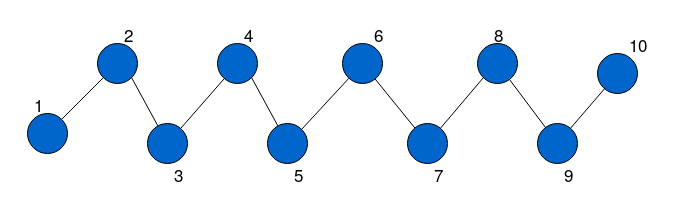
\includegraphics[width=\textwidth]{images/path-graph-dif.png}
		\caption{}
		\label{path-network}
	\end{subfigure}~
	\begin{subfigure}[b]{0.45\textwidth}
		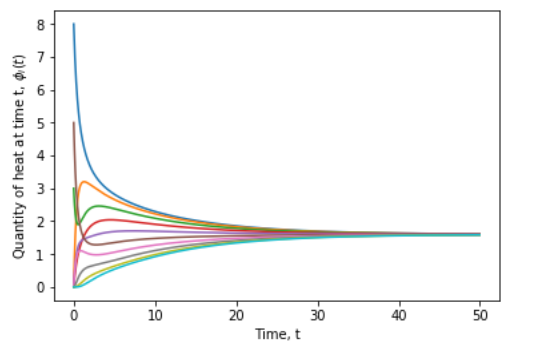
\includegraphics[width= \textwidth]{images/path-network-diffusion.png}
		\caption{}
		\label{dif-path-network}
	\end{subfigure}\\
	\begin{subfigure}[b]{0.37\textwidth}
		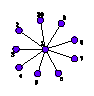
\includegraphics[width=\textwidth]{images/star-difusion.pdf}
		\caption{}
		\label{stardifn-graph}
	\end{subfigure}~
	\begin{subfigure}[b]{0.45\textwidth}
		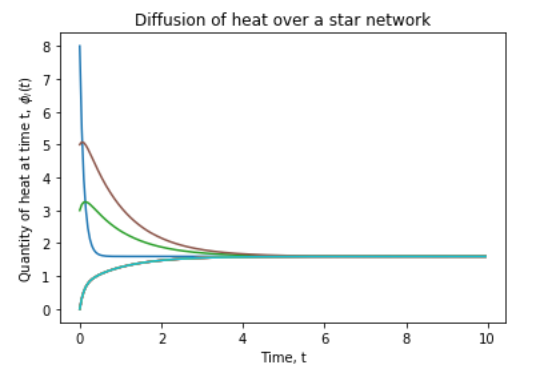
\includegraphics[width= \textwidth]{images/star-quantity-time.png}
		\caption{}
		\label{stardifn-plot}
	\end{subfigure}\\
	\begin{subfigure}[b]{0.37\textwidth}
		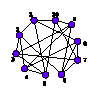
\includegraphics[width=\textwidth]{images/regular-dif.pdf}
		\caption{}
		\label{regdifn-graph}
	\end{subfigure}~
	\begin{subfigure}[b]{0.45\textwidth}
		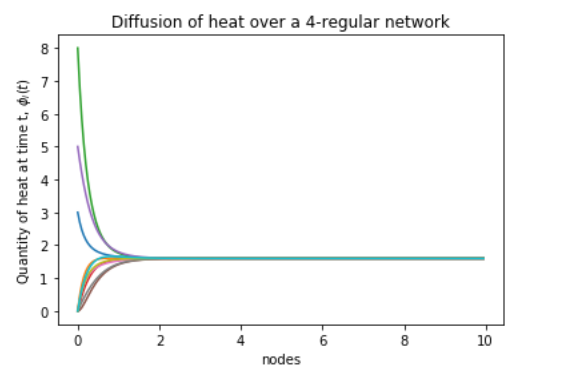
\includegraphics[width= \textwidth]{images/regular-quantity-time.png}
		\caption{}
		\label{regdifn-plot}
	\end{subfigure} 
   \caption{The figures are illustrations in the first column are the different networks that is at the top is the path network, followed by star network and lastly $4-$ regular network. The second column consist of the plots of diffusion of quantities against time. Each figure in the second column corresponds to the network in the first column.}
   \label{dif-diff-networks}
\end{figure}

On comparing the diffusion over the $3$ types of networks, we observe that it takes quite a long time for equilibrium to be attained in path network compared to the star and regular network. The equilibrium times are $t= 40, 5,$ and $2$ for the path, star and $4$-regular networks respectively.   
In the regular network, the number of direct interactions among nodes is quite high and so are the long range interactions compared to the star and path network. This partially explains why diffusion occurs much faster in the regular network than in the other two networks of the same size. However, as discussed before, the quantity of heat at each node at equilibrium in all networks is the same value of $1.6$ which is the average of the quantities assigned to all nodes initially which cements the fact that the structure of the network has no influence on the quantity at equilibrium.

A better visualisation of the diffusion process over the star network in Fig.~\ref{dif-diff-networks}(\subref{stardifn-graph}) at different time intervals is illustrated in Fig.~\ref{visualise} where the quantity of heat at any node at time $t$ is proportional to the size of the node.

\begin{figure}[!h]
	\centering
	\begin{subfigure}[b]{0.38\textwidth}
		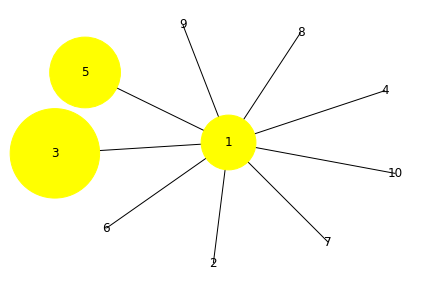
\includegraphics[width=\textwidth]{images/star-t-0.png}
		\caption{$t=0$}
		\label{t0}
	\end{subfigure}~
	\begin{subfigure}[b]{0.38\textwidth}
		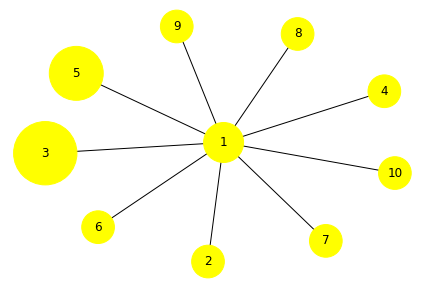
\includegraphics[width= \textwidth]{images/star-t-1.png}
		\caption{$t=1$}
		\label{t1}
	\end{subfigure}\\
	\begin{subfigure}[b]{0.38\textwidth}
		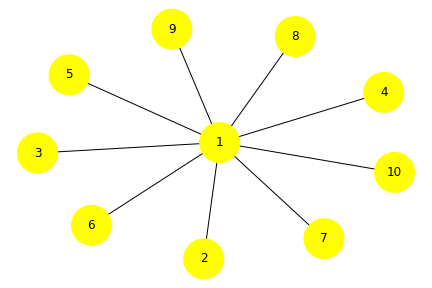
\includegraphics[width=\textwidth]{images/star-t-6.png}
		\caption{$t=6$}
		\label{t6}
	\end{subfigure}~
	\begin{subfigure}[b]{0.38\textwidth}
		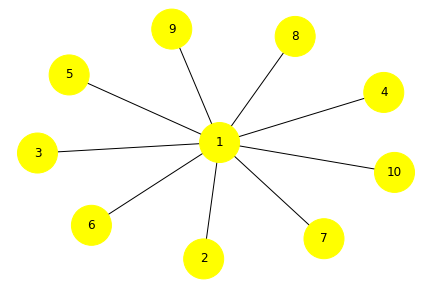
\includegraphics[width= \textwidth]{images/star-t-9.png}
		\caption{$t=9$}
		\label{t9}
	\end{subfigure}
	\caption{Initially (t=0), all nodes are assigned certain quantities of heat according to the vector $\mathbf{\phi_0} = [3,0,8,0,5,2,0,0,0,2]$ where by the size of the node is proportional to the heat quantity that node has. Figures (\subref{t0}), (\subref{t1}), (\subref{t6}), and (\subref{t9}) depict the status of the networks at $t=0$, $t=1$, $t=6$, and $t=9$ respectively.}
	\label{visualise}
\end{figure}

\newpage
\section{Impact of Structure on the rate of diffusion}
The structure of a network basically means the way in which nodes are connected in the network. For instance, in a regular network each node is connected to equal number of nodes, for a star network one node is positioned in a way that all other nodes are connected to it.
Let us consider two structures of networks that manifest in many artificial and real world networks.  First, the Erdos-Renyi (ER) network in which a pair of nodes is connected by random probability, $p$. The degree of nodes in ER network follow a Poisson distribution \cite{erdos1960evolution}. Second, we consider the Barabasi-Albert(BA) network in which connection of nodes follows scale free power-law distribution, that is to say, the probability of finding a node with degree $k$ decreases as the negative power of $k$. It therefore less likely to find a node with high degree (hub) compared to low degrees \cite{barabasi1999emergence, estrada2011structure} . 
Consider ER and BA networks with $n=100$ and average degree $\bar{k}= 6$, we randomly assign quantities(range of 0 to 20) of heat to each node and allow diffusion to occur at different values of conductance $x$. After every time step $t$,we compute the quantities at each node as depicted in Figure \ref{barabasi-Erdos-compare}.
 
%\newpage
\begin{figure}[H]
	\centering
	\begin{subfigure}[b]{0.45\textwidth}
		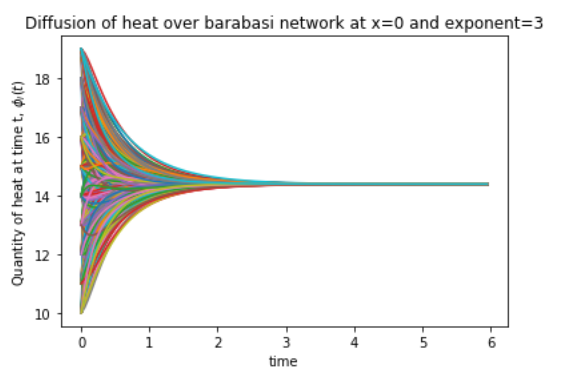
\includegraphics[width=\textwidth]{images/barabasi-x0.png}
		\caption{$x=0$}
		\label{barabasi-x0}
	\end{subfigure}~
	\begin{subfigure}[b]{0.45\textwidth}
		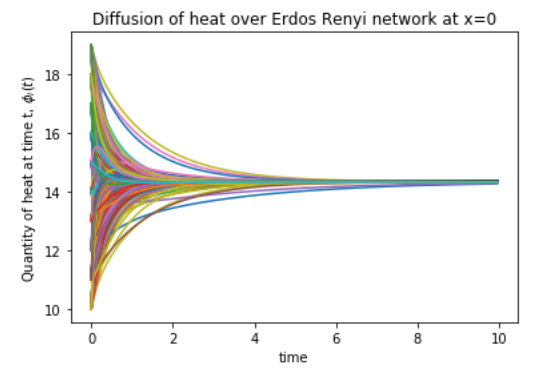
\includegraphics[width= \textwidth]{images/erdos-x0.png}
		\caption{$x=0$}
		\label{erdos-x01}
	\end{subfigure}\\
	\begin{subfigure}[b]{0.45\textwidth}
		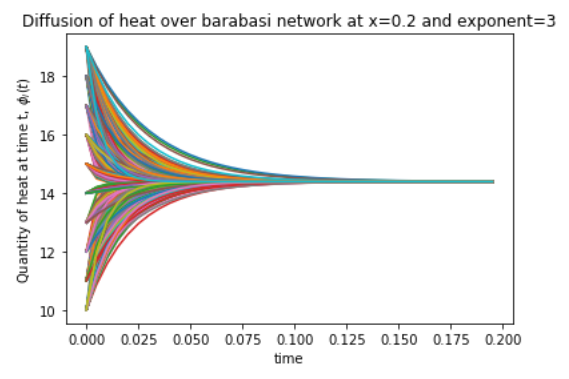
\includegraphics[width= \textwidth]{images/barabasi-x02.png}
		\caption{$x=0.2$}
		\label{barabasi-x02}
	\end{subfigure}~
	\begin{subfigure}[b]{0.45\textwidth}
		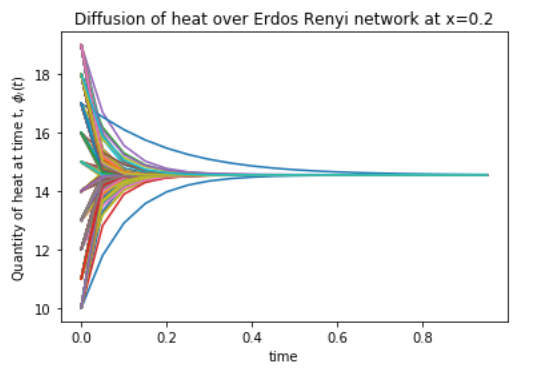
\includegraphics[width= \textwidth]{images/erdos-x02.png}
		\caption{$x=0.2$}
		\label{erdos-x02}
	\end{subfigure}\\
	\begin{subfigure}[b]{0.45\textwidth}
		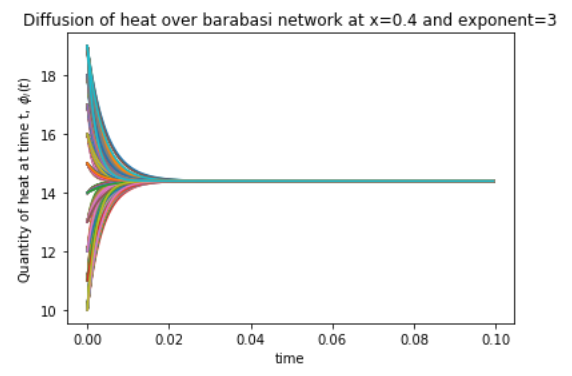
\includegraphics[width= \textwidth]{images/barabasi-x04.png}
		\caption{$x=0.4$}
		\label{barabasi-x04}
	\end{subfigure}~
	\begin{subfigure}[b]{0.45\textwidth}
		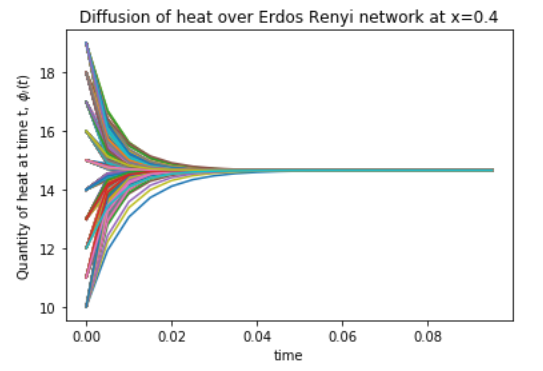
\includegraphics[width= \textwidth]{images/erdos-x04.png}
		\caption{$x=0.4$}
		\label{erdos-x04}
	\end{subfigure}
	\caption{Barabasi networks (left) and Erdos Renyi networks(right) of 1000 nodes and average degree of 6. Top row is illustration of diffusion process at $x=0$ ( i.e accounting for direct interactions only), middle row corresponds to $x=0.2$ followed by $x=0.4$ in the last row}
	\label{barabasi-Erdos-compare}
\end{figure}

From Fig \ref{barabasi-Erdos-compare} at the top row, we observe that at $x=0$, equilibrium is reached faster for Barabasi-Alberto(BA) network ( that is after about $4$ time steps) compared to Erdos-Renyi(ER) network in which equilibrium is reached after about $10$ time steps. This is explained based on the fact that in BA networks there are more hubs compared to ER networks. These hubs tend to interact with a number of nodes with in the network thus fastening the diffusion process. On increasing $x$ to $0.2$, we observe a drastic drop in equilibrium time from  $4$ to $0.15$ time steps and from $10$ to $0.8$ time steps for BA and ER networks respectively. It is important to note that drop in equilibrium time is relatively higher in ER than in BA and this is because of the few hubs in ER networks which aids a larger number of long range interactions than in BA networks. As $x$ increases further to $0.4$, equilibrium time further drops to $0.03$ and $0.06$ for BA and ER networks respectively.

\section{Influence of Heterogeneity on Diffusion over network}
The heterogeneity of a network is the irregularity characterised by the existence of a nodes with degree significantly larger than the average degree of the network \cite{estrada2010quantifying,albert2002statistical,newman2003structure}.
The quantification of heterogeneity is one the areas where tremendous research has been on going and various measures have been introduced \cite{estrada2010quantifying}.
Here, we consider heterogeneity in scale free networks with $n=1000$ and average degree $\bar{k}=20$ by varying power exponent, $\gamma$. For different conductances $x$, we assign initial quantities of heat to each of the $200$ nodes with highest degree. Figure \ref{quantity-exponents} illustrates how the average quantities of heat of the selected initial diffusion nodes varies with time.
\begin{figure}[!h]
	\centering
	\begin{subfigure}[b]{0.32\textwidth}
		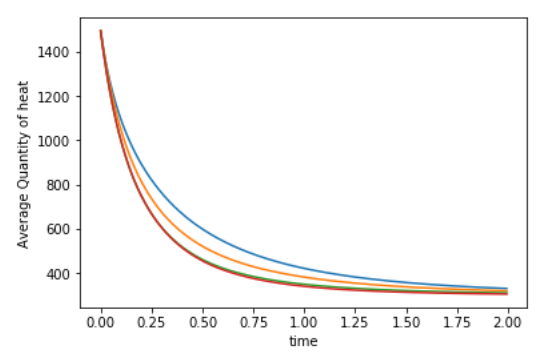
\includegraphics[width=\textwidth]{images/quantity-time-exponents-x0.png}
		%\caption{$x=0.1, t=0$}
		%\label{gridt0x01}
	\end{subfigure}~
	\begin{subfigure}[b]{0.32\textwidth}
		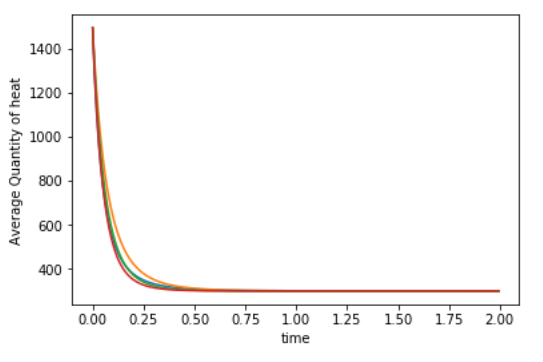
\includegraphics[width= \textwidth]{images/quantity-time-exponents-x01.png}
		%\caption{$x=0.1, t=0.5$}
		%\label{gridt05x01}
	\end{subfigure}~
	\begin{subfigure}[b]{0.32\textwidth}
		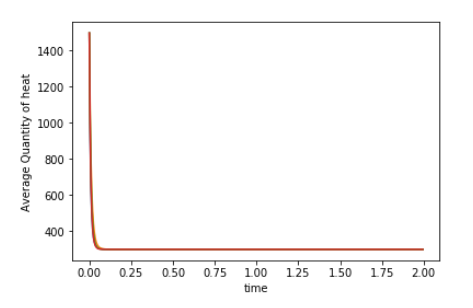
\includegraphics[width= \textwidth]{images/quantity-time-exponents-x03.png}
		%\caption{$x=0.1, t=3.0$}
		%\label{gridt3x01}
	\end{subfigure} \\
	\begin{subfigure}[b]{0.80\textwidth}
		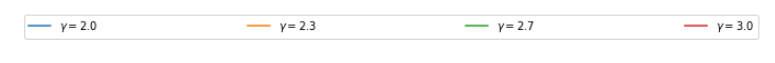
\includegraphics[width= \textwidth]{images/legend-gamma.png}
	\end{subfigure}
	\caption{Plots of the average quantity of heat for $200$ nodes with the highest degree centrality against time for $3$ scale free networks having different values of the power exponent($2.0$,$2.3$,$2.7$, and $3.0$), n=1000 and average degree=$6$. The figures to the left, centre and right correspond to x values $0$,$0.1$, and $0.3$ respectively.}
	\label{quantity-exponents}
\end{figure}

%\begin{figure}[!h]
%	\centering
%	\begin{subfigure}[b]{0.45\textwidth}
%		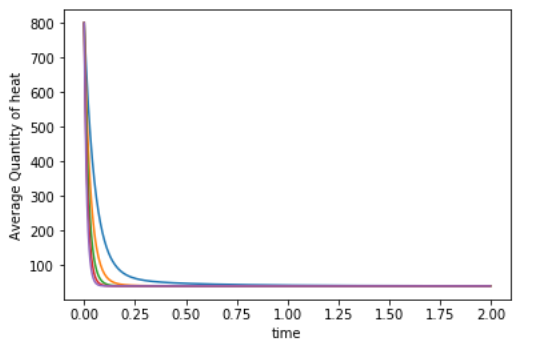
\includegraphics[width=\textwidth]{images/Barabasi-highest-degree.png}
%		%\caption{$x=0.1, t=0$}
%		%\label{gridt0x01}
%	\end{subfigure}~
%	\begin{subfigure}[b]{0.45\textwidth}
%		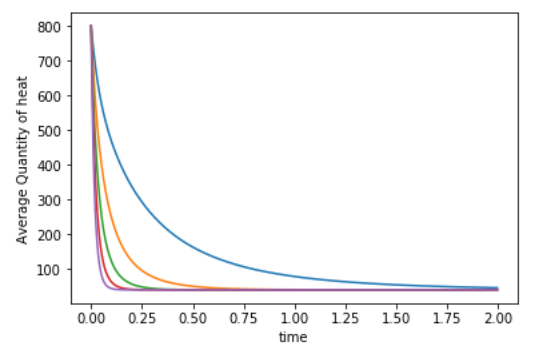
\includegraphics[width= \textwidth]{images/barabasi-random-selection.png}
%		%\caption{$x=0.1, t=0.5$}
%		%\label{gridt05x01}
%	\end{subfigure}
%	\caption{Illustration of the impact of the choice of the initial nodes from which diffusion starts. We consider Barabasi-Albert networks of $100$ nodes. The left plot corresponds to one in which the $5$ most important node according to degree centrality(hubs) are chosen. On the other hand, the plot at the right is as a result of random selection of initial nodes. }
%	\label{}
%\end{figure}

\newpage
\section{Impact of choice of Initial diffusion nodes on the diffusion process on networks}
%We take a Barabasi-Albert network and Erdos-Renyi network, both of 100 nodes and average of 6. We choose $5$ nodes with the highest degree centrality to which we assign specific amounts of heat. At each time $t$, we measure the average quantity of heat at the $5$ nodes as illustrated by figure. 

\begin{figure}[!h]
	\centering
	\begin{subfigure}[b]{0.45\textwidth}
		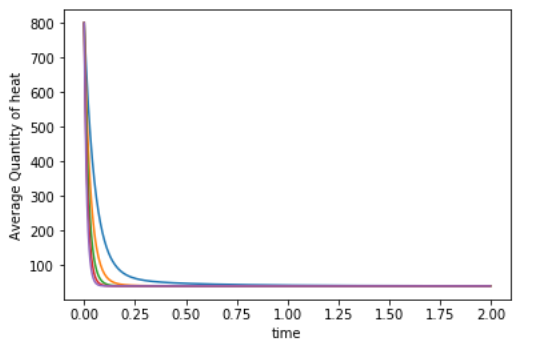
\includegraphics[width= \textwidth]{images/Barabasi-highest-degree.png}
		\caption{}
		\label{}
	\end{subfigure}~
	\begin{subfigure}[b]{0.45\textwidth}
		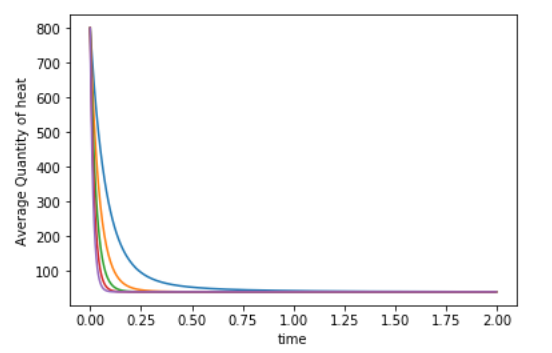
\includegraphics[width= \textwidth]{images/E-R-largest.png}
		\caption{}
		\label{}
	\end{subfigure}\\
    \begin{subfigure}[b]{0.45\textwidth}
    	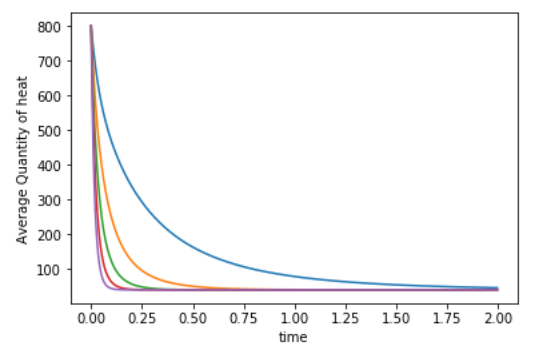
\includegraphics[width= \textwidth]{images/barabasi-random-selection.png}
    	\caption{}
    	\label{}
    \end{subfigure}~
    \begin{subfigure}[b]{0.45\textwidth}
    	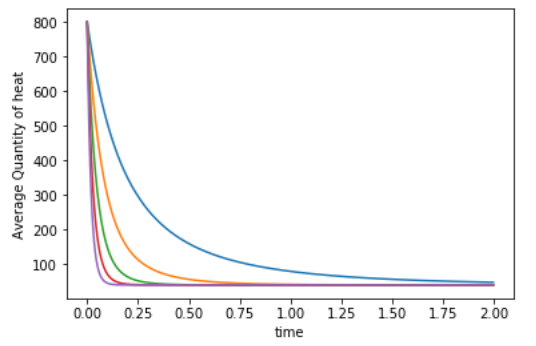
\includegraphics[width= \textwidth]{images/E-R-random.png}
    	\caption{}
    	\label{}
    \end{subfigure}
    \caption{ Results of the simulations for two networks. One is the Barabasi-Albert(BA) network and  the other is Erdos-Renyi(ER) network, both of $100$ nodes and average degree of $6$. Taking $5$ of the most important (by degree) nodes in the network from which diffusion is initiated by assigning certain quantities of heat to those nodes, the simulation of the diffusion is illustrated in plots (a) and (b) for the BA and ER networks respectively.}
    \label{key}
\end{figure}

We observe that in BA network, heat spreads quite faster than in ER network that is to say by $t=0.6$, all the $5$ hubs in BA have levelled to equal amount while for ER, nodes still have un equal amounts of heat. This is because we assign quantities of heat to $5$ hubs of a network and they quickly spread heat to other nodes compared to ER where there are relatively fewer hubs among the five chosen nodes to initiate the diffusion process.

\newpage
\section{Spectrum of the Generalised Laplacian matrix}
The spectrum of the Laplacian matrix is the set of eigenvalues and their multiplicities \cite{estrada2011epidemic}. Let $\lambda_1 < \lambda_2 < \cdots < \lambda_n$ be the eigenvalues of $L(x)$ and their corresponding multiplicities $m(\lambda_1), m(\lambda_2), \cdots, m(\lambda_n)$. The spectrum of $L$ is given by
\begin{equation}
S_p L = \big(\lambda_1 \quad \lambda_2 \quad \cdots \quad \lambda_n \\
m(\lambda_1) \quad m(\lambda_2) \quad \cdots \quad m(\lambda_n)  \big).
\end{equation}
Some analytical expressions for the spectra of the Laplacian matrix of some common simple networks are:\\
\begin{itemize}
	\item Star, $S_n$: $S_p(L) = {0~ 1^{n-2}~ n}$\\
	\item Path, $P_n$: $S_p(L) = {2-2\cos\big( \frac{\pi(j-1)}{n}\big) }$
\end{itemize}
For generalised Laplacian matrix $L(x)$, the above expressions as a function of conductance $x$ are given by
\begin{itemize}
	\item Star, $S_n$: $S_p(L(x)) = {0~ (1+8x)^{n-2}~ n}$\\
	\item Path, $P_n$: $S_p(L(x)) = { }$
\end{itemize}
\begin{figure}[!h]
	\centering
	\begin{subfigure}[b]{0.45\textwidth}
		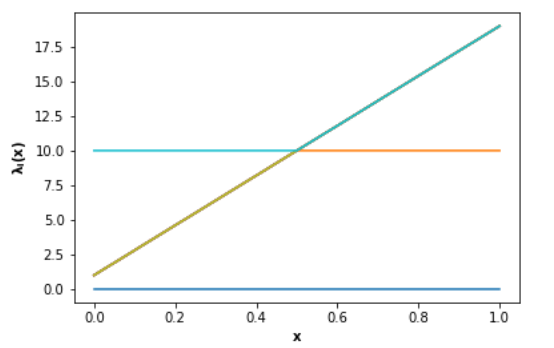
\includegraphics[width= \textwidth]{images/Star-network-eigenplot.png}
		%\caption{$x=0.1, t=0.5$}
		\label{star-spectra}
	\end{subfigure}~
	\begin{subfigure}[b]{0.45\textwidth}
		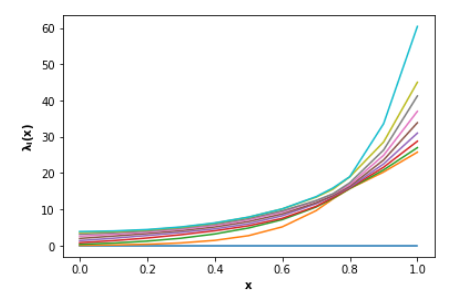
\includegraphics[width= \textwidth]{images/Path-network-eigenplot.png}
		%\caption{$x=0.1, t=3.0$}
		\label{path-spectra}
	\end{subfigure} \\
	\begin{subfigure}[b]{0.85\textwidth}
		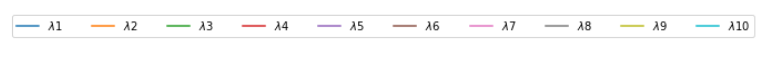
\includegraphics[width= \textwidth]{images/legend-eigenvalues.png}
		%\caption{$x=0.1, t=3.0$}
		%\label{gridt3x01}
	\end{subfigure}
	\caption{Illustrations of variation of eigenvalues with conductance $x$ two networks. The first figure from the left a star network, $S_{10}$ (in Fig. \ref{stardifn-graph}) and the other is a path network. Both networks have $10$ nodes each.}
	\label{eigen-xvalues}
\end{figure}
As discussed before, the eigenvalues $\lambda_i(x)$ of the Laplacian matrix $L(x)$ are an increasing function of $x$ except for the smallest eigenvalue $\lambda_1(x) = 0$ which remains almost constant as observed in Figure \ref{eigen-xvalues}. For the star network , both $\lambda_1(x) = 0$ and $\lambda_1(n) = 5$ remain constant the analytical expressions mentioned before. However, the rest of the eigenvalues increase linearly with increase in $x$ values. At $x=0.5$, we observe that all eigenvalues are equal with a value of $10$. This is because at $x=0.5$, all edges of the star network have a weight of $1$ and thus, a complete network,$K_n$, whose spectrum is given by $S_p(L) = \{0~ n^{n-1} \}$. On the other hand, the path network follows a similar trend as that of the star network but the $x$ value at which all eigenvalues (except $\lambda_i=0$) are equal is relatively higher than $0.5$ that is to say the point lies at $x=0.7$. 

\newpage

\section{Diffusion process on a grid}
We consider a 2-dimensional discrete grid in which each point is connected to 8 of its nearest neighbours. Initially, we assign heat quantities to all the points on the grid and then we investigate how the diffusion process occurs and at each time $t$, we compute the quantity of heat at each node using equation \ref{dif-final-eqn}. \\
Let us take a 20 by 20 grid on which we assigned heat quantities of amounts 5, 7 and 10 to a few points and the rest are assigned zero. The figures below illustrate the diffusion process in which both the direct and long range interactions are accounted for at different values of x.
\begin{figure}[!h]
	\centering
	\begin{subfigure}[b]{0.25\textwidth}
		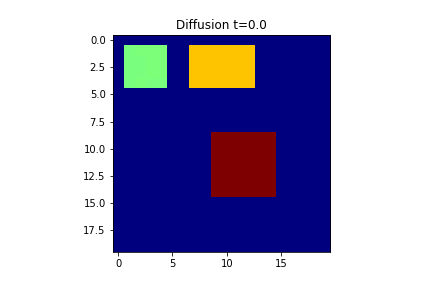
\includegraphics[width=\textwidth]{images/grid-t0-x0.png}
		%\caption{$x=0, t=0$}
		%\label{gridt0x0}
	\end{subfigure}~
	\begin{subfigure}[b]{0.25\textwidth}
		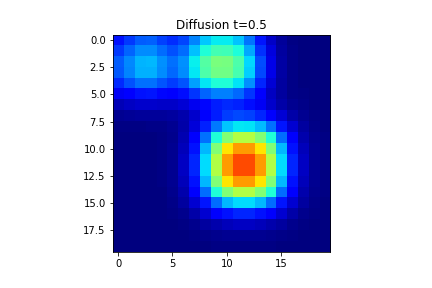
\includegraphics[width= \textwidth]{images/grid-t05-x0.png}
		%\caption{$x=0, t=0.5$}
		%\label{gridt05x01}
	\end{subfigure}~
    \begin{subfigure}[b]{0.25\textwidth}
    	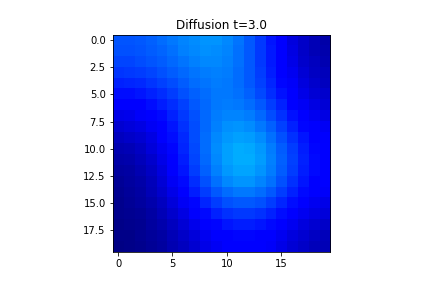
\includegraphics[width= \textwidth]{images/grid-t3-x0.png}
    	%\caption{$x=0, t=3.0$}
    	%\label{gridt3x01}
    \end{subfigure}~
    \begin{subfigure}[b]{0.25\textwidth}
    	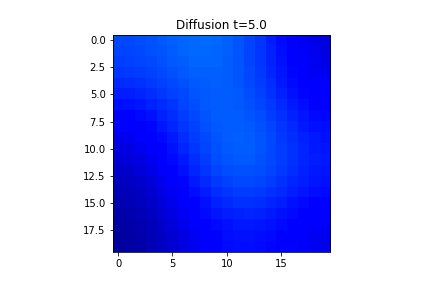
\includegraphics[width= \textwidth]{images/grid-t5-x0.png}
    	%\caption{$x=0, t=5.0$}
    	%\label{gridt5x01}
    \end{subfigure}
%\caption{Sample illustrations for progression of diffusion for $x=0$ i.e direct interactions only.}
%\label{gridatx0}
\end{figure}

\begin{figure}[!h]
	\centering
	\begin{subfigure}[b]{0.25\textwidth}
		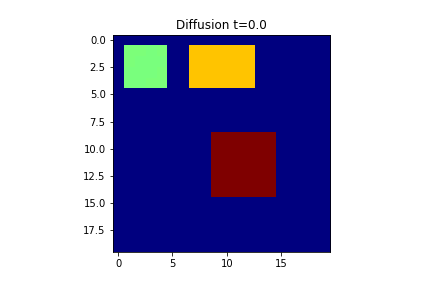
\includegraphics[width=\textwidth]{images/grid-t0-x01.png}
		%\caption{$x=0.1, t=0$}
		%\label{gridt0x01}
	\end{subfigure}~
	\begin{subfigure}[b]{0.25\textwidth}
		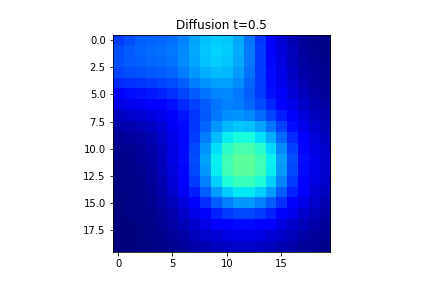
\includegraphics[width= \textwidth]{images/grid-t05-x01.png}
		%\caption{}
		%\label{}
	\end{subfigure}~
	\begin{subfigure}[b]{0.25\textwidth}
		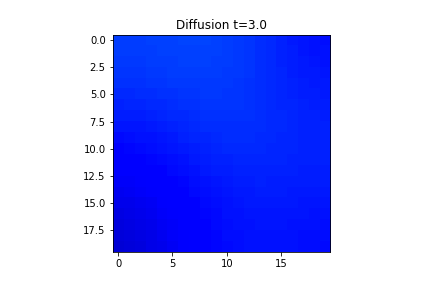
\includegraphics[width= \textwidth]{images/grid-t3-x01.png}
		%\caption{}
		%\label{}
	\end{subfigure}~
	\begin{subfigure}[b]{0.25\textwidth}
		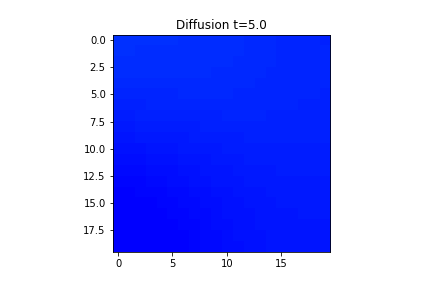
\includegraphics[width= \textwidth]{images/grid-t5-x01.png}
		%\caption{}
		%\label{}
	\end{subfigure}
\end{figure}

\begin{figure}[!h]
	\centering
	\begin{subfigure}[b]{0.25\textwidth}
		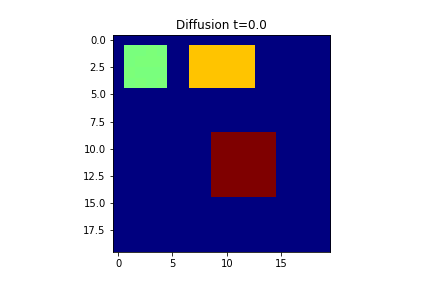
\includegraphics[width=\textwidth]{images/grid-t0-x02.png}
		%\caption{$x=0.2, t=0$}
		%\label{gridt0x02}
	\end{subfigure}~
	\begin{subfigure}[b]{0.25\textwidth}
		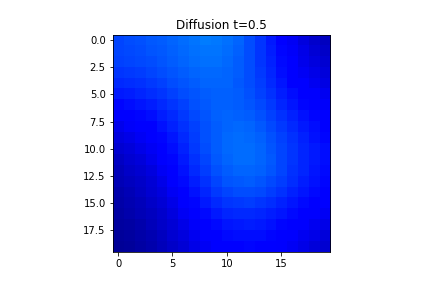
\includegraphics[width= \textwidth]{images/grid-t05-x02.png}
		%\caption{$x=0.2, t=0.5$}
		%\label{gridt05x02}
	\end{subfigure}~
	\begin{subfigure}[b]{0.25\textwidth}
		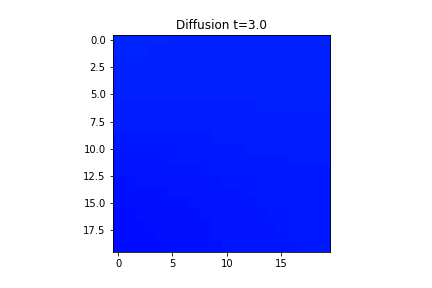
\includegraphics[width= \textwidth]{images/grid-t3-x02.png}
		%\caption{$x=0.2, t=3.0$}
		%\label{gridt2x02}
	\end{subfigure}~
	\begin{subfigure}[b]{0.25\textwidth}
		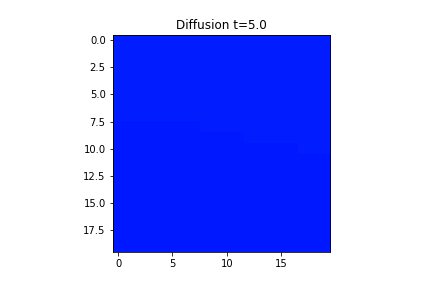
\includegraphics[width= \textwidth]{images/grid-t5-x02.png}
		%\caption{$x=0.2, t=5.0$}
		%\label{gridt3x02}
	\end{subfigure}\\
\vspace{0.25cm}
	 \begin{subfigure}[b]{0.60\textwidth}
	 	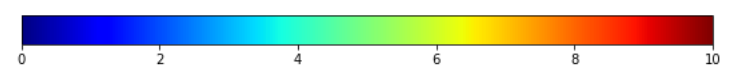
\includegraphics[width= \textwidth]{images/colour-bar-grid.png}
	 \end{subfigure}
\caption{Illustrations for diffusion over a grid. The upper most row corresponds to diffusion when only direct interactions among neighbouring nodes are accounted for. The middle and last row are results obtained when long range interactions are included at $x=0.1$ and $x=0.2$ respectively. The intensity of heat follows a color grid where by red implies higher intensity followed by yellow and blue implies low heat intensities.}
\label{diffusionongrid}
\end{figure}

At $t=0$, diffusion on the grid starts off with $3$ strong regions having high quantities of heat as shown in Figure \ref{diffusionongrid} in first column of the top, middle and bottom rows which correspond to $x$ values of $0$, $0.1$ and $0.2$ respectively. As the diffusion process continues, we see that at $t=0.5$, strong heat points can still be spotted for $x=0$, relatively strong points in $x=0.1$ and almost complete diffusion in $x=0.2$. we can also see that by $t=2.0$, heat is uniformly distributed across the grid for $x=0.1$ and $x=0.2$. However, for $x=0$ diffusion is still ongoing and we can notice strong heat points at the centre of the grid. Following the sequences in the figures, we can conclude that as $x$ (i.e increase in intensity of long range interactions), the diffusion process goes faster and equilibrium across the grid is reached faster as observed in the above simulations where for $x=0.2$,$x=0.1$ equilibrium is reached by $t=3$ while for $x=0$, equilibrium is not yet reached by then.

\nocite{*}
\bibliographystyle{abbrv}
\bibliography{references}
\end{document}
